\chapter{Une première implémentation}

\section{Motivation}

La première implantation a été faite sous Python avec pour but principal de rester le plus proche possible de l'architecture neuronale du réseau pour mieux étudier le fonctionnement de l'algorithme d'apprentissage. Quitte à perdre en rapidité de calcul, nous avons ainsi décidé de créer des objets neurones et un réseau composé de plusieurs de ces neurones. Nous avons alors pu appliquer cette implémentation sur des cas simples (XOR notamment, \autoref{sec:Résultats}), mais aussi obtenir un aperçu des optimisations possibles afin d'accélérer les calculs. Cela s'est effectivement rapidement révélé nécessaire.  

\section{Diagramme UML}

Le diagramme UML (figure \ref{Diagramme UML des classes Neuron et Network}) comporte ainsi deux classes principales : une classe Neuron et une classe Network. 

Le neurone a été défini comme une entité autonome, qui comporte des entrées et une sortie et est caractérisé par des poids ainsi que ses relations avec d'autres neurones (parents ou enfants). Il peut alors calculer la sortie si les sorties de ses parents ont préalablement été évaluées. Réciproquement, pour calculer le gradient de l'erreur par rapport à chacun de ses poids, il a tout d'abord besoin de ceux de ses enfants.


\begin{figure}
\begin{center}
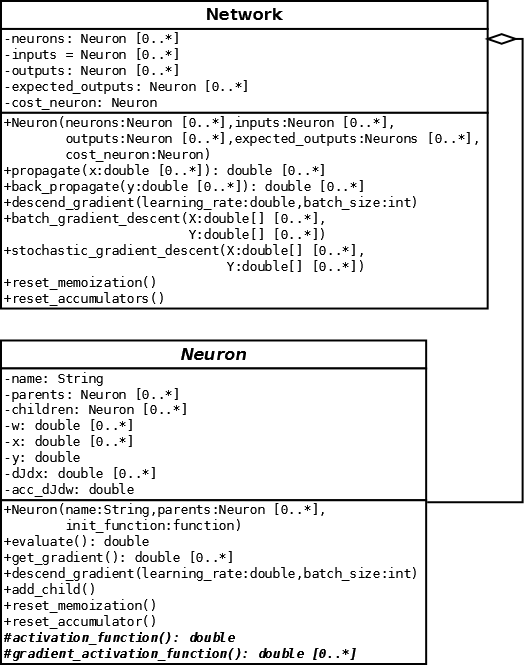
\includegraphics[scale=0.3]{images/uml_simplifie_maispastrop_imp1.png}
\caption{Diagramme UML des classes Neuron et Network}
\label{Diagramme UML des classes Neuron et Network}
\end{center}
\end{figure}

On répartit les neurones en différentes catégories selon leurs fonctions d'activation (sigmoïde, tangente hyperbolique, Softmax ou ReLu par exemple).

Ainsi la classe Neuron possède de nombreuses sous-classes correspondant à ces fonctions. En outre, il existe plusieurs sous-classes destinées aux neurones ayant un comportement particulier. On distingue BiasNeuron, qui permet d'ajouter un biais au niveau des entrées d'un autre neurone, et InputNeuron correspondant simplement aux neurones d'entrées. L'ajout d'un neurone de coût (costNeuron) à la fin du réseau permet de calculer directement l'erreur lors de la propagation d'une entrée. Il faudra ainsi spécifier pour chaque entrée la sortie attendue pour calculer le coût (avec un InputNeuron).

\begin{figure}
\begin{center}
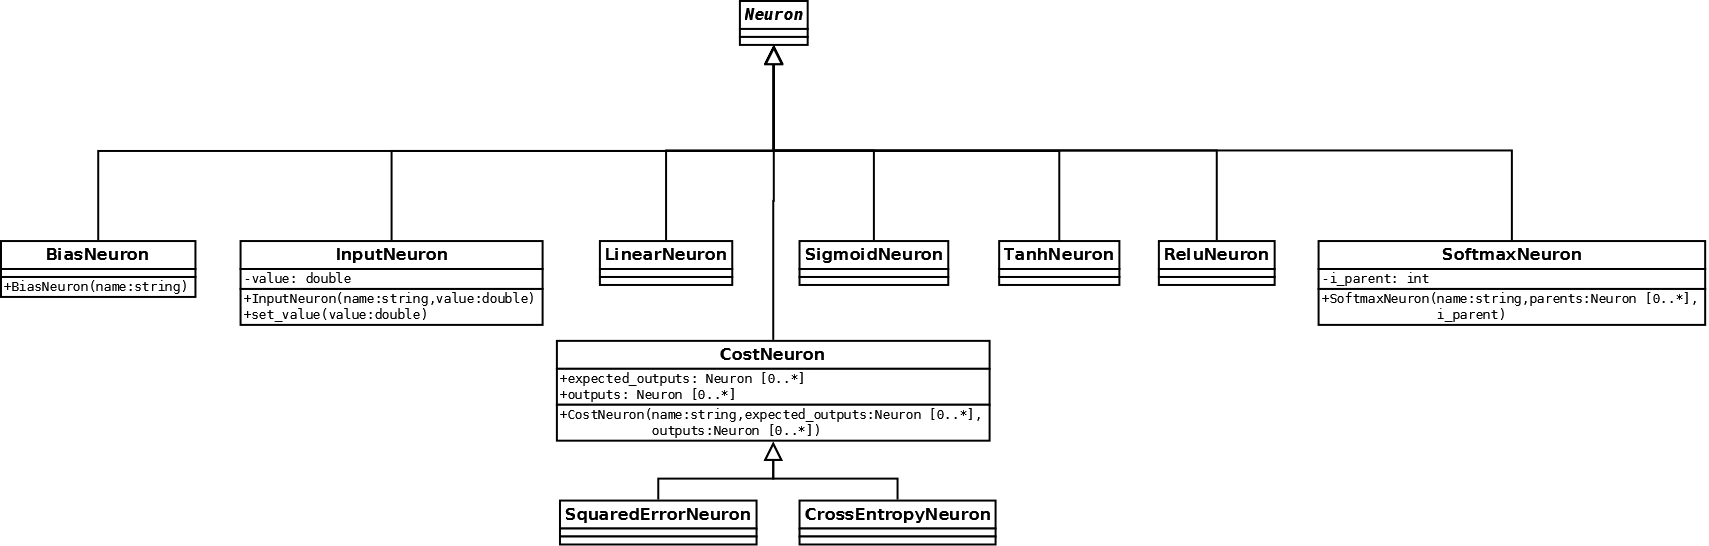
\includegraphics[scale=0.18]{images/uml_neurone_imp1.png}
\caption{Hiérarchie de la classe Neuron}
\label{uml_neurone_imp1}
\end{center}
\end{figure}


Les liens entre neurones ne seront pas mémorisés par le réseau. Cette tâche sera réalisée par les neurones eux-mêmes. Ainsi, chacun possédera en attribut une liste de parents et une liste d'enfants, ce qui lui permettra de se situer dans le réseau. Ces deux listes sont indispensables afin de propager le résultat de sortie du neurone et afin de rétropropager le gradient lors de l'algorithme d'apprentissage.
	
\section{Principe de fonctionnement}
Pour créer un réseau de neurones, on commence par créer les différents neurones (InputNeuron, SigmoidNeuron, CrossEntropyNeuron, ...) en spécifiant les parents à chaque fois. Le programme mettra lui-même à jour les listes de parents et d'enfants de chaque neurone au fur et à mesure qu'on en ajoute de nouveaux afin de créer les différentes relations entre neurones. On crée finalement le réseau (Network) en spécifiant les entrées, sorties, le neurone de coût et les neurones intermédiaires.
On peut alors appliquer deux fonctions principales sur le réseau. "Propagate" permet de calculer la sortie du réseau pour une entrée fournie en paramètre. "Batch\_propagation\_descent" permet d'appliquer l'algorithme de d'apprentissage basée sur la backpropagation du gradient pour un ensemble d'entrées, de sorties attendues et un learning rate $\eta$ donnés. 
Pour réaliser cet algorithme d'apprentissage, le programme sélectionne une entrée x et une sortie attendue y\_expected. Il applique ensuite "propagate" afin d'obtenir la sortie y et le coût correspondant. "backpropagate" permet alors de faire remonter le gradient jusqu'à chaque neurone où il sera accumulé dans une variable acc\_dJdw. On réitère ce processus pour tous les couples x et y\_expected. Enfin, on met à jour les poids grâce à un "descent\_gradient" à l'aide de l'équation \ref{mise_a_jour_poids_batch} (valable pour un batch) :

\begin{equation}
w(t+1) = w(t) - \frac{\eta}{batch\_size}acc\_dJdw
\label{mise_a_jour_poids_batch}
\end{equation}

Nous avons utilisé diverses astuces afin d'améliorer l'efficacité de notre programme. Par exemple, la sigmoide est une fonction d'activation souvent utilisée. Elle est définie par $f(x) = \frac{1}{1+\exp(-x)}$. Au lieu d'entrer directement la formule complète de la dérivée, nous la simplifions en l'écrivant sous la forme $f'(x) = f(x) * (1 - f(x))$.
Nous utilisons deux variables acc\_dJdw et dJdx dans chaque neurone. La première permet d'accumuler les corrections à apporter aux poids que l'on applique à la fin du batch. dJdx sert de mémoïsation afin d'optimiser les calculs et de ne pas en faire d'inutiles. En effet, pour calculer son gradient, chaque neurone a besoin des gradients de ses enfants. Si nous ne mémorisions pas le gradient de chaque neurone dans dJdx, nous devrions le recalculer à chaque fois qu'un des parents le demande. Cela alourdirait énormément les calculs et ferait augmenter significativement le temps d'exécution. Ces deux variables doivent évidemment être réinitialisées à la fin du passage du batch de données.

\section{Résultats}
\label{sec:Résultats}
Afin de tester le fonctionnement de cette première implémentation, nous avons commencé sur un modèle simple: le XOR. Le but était donc de réaliser un réseau de neurones à deux entrées et une sortie qui fonctionne comme un XOR : il renvoie $0$ si les entrées sont semblables (toutes deux égales à un ou à zéro) et il renvoie $1$ si elles sont différentes (l'une égale à un et l'autre à zéro). On entraine alors le réseau sur le batch définissant le XOR : les quatre couples $((0,0),0)$, $((0,1),1)$, $((1,0),1)$ et $((1,1),0)$. Le gradient est alors calculé en moyennant les résultats du réseau sur ces quatre entrées.
Cela a permis de valider le bon fonctionnement de l'implémentation.

Des premiers tests ont été réalisés avec un réseau possédant une couche cachée de deux neurones. Les résultats sont alors plutôt mauvais : alors que théoriquement le XOR est réalisable avec cette architecture, nous avons pu observer que lors de l'exécution de l'algorithme, la descente du gradient a tendance à se bloquer dans un minimum local de la fonction de coût. 

\begin{figure}[!h]
\begin{center}
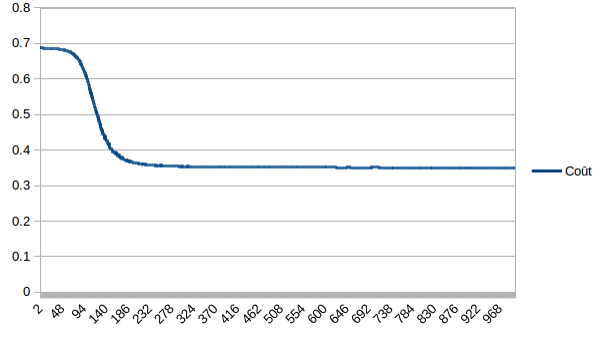
\includegraphics[scale=0.6]{images/xor_cost_function.png}
\caption{fonction de coût bloquée dans un minimum local}
\label{xor_cout_bloque}
\end{center}
\end{figure}

Nous avons alors pu remarquer que même en modifiant différents paramètres, (valeurs initiales des poids, learning rate ou les fonctions d'activation), cela restait inefficace, et les résultats obtenus ne correspondaient pas à la fonction xor que l'on attendait (voir figure \ref{xor_non_fonctionnel}).

\begin{figure}[!h]
\begin{center}
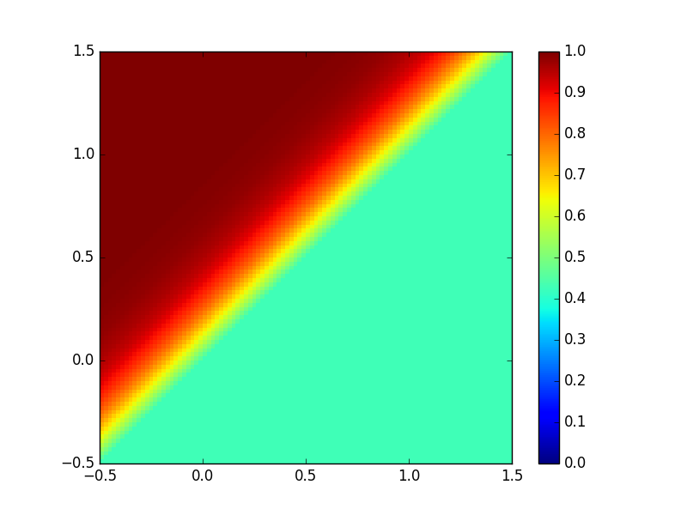
\includegraphics[scale=0.6]{images/xor_non_fonctionnel.png}
\caption{XOR bloqué dans un minimum local}
\label{xor_non_fonctionnel}
\end{center}
\end{figure}

Nous sommes alors passés sur une seconde architecture avec cette fois quatre neurones dans la couche cachée. On obtient cette fois de très bons résultats comme celui de la figure \ref{xor_relu_2_4}.

\begin{figure}[!h]
\begin{center}
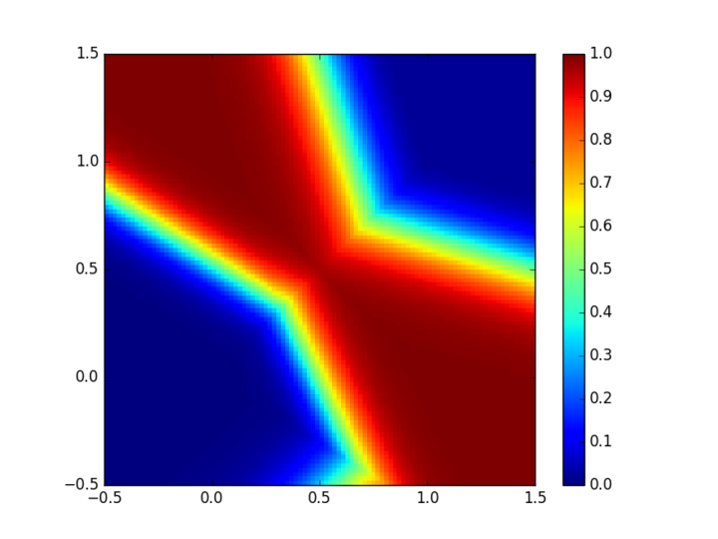
\includegraphics[scale=0.6]{images/xor_relu_2_4.png}
\caption{2 couches cachées de 4 neurones-ReLu}
\label{xor_relu_2_4}
\end{center}
\end{figure}

On peut remarquer avec cette présentation des résultats que le réseau de neurones renvoie les bonnes réponses du XOR pour les entrées définies pour l'entrainement. Pour toutes les autres valeurs,  le réseau "interprète" alors avec son apprentissage. On peut remarquer que cette interprétation varie selon la fonction d'activation. Ainsi pour la tangente hyperbolique les zones définies sont beaucoup plus courbées que pour la ReLu, comme le montre la figure \ref{xor_tanh_2_4}. On peut lier cela avec les représentations graphiques de ces fonctions. En effet la fonction Relu est en fait deux demi-droites alors que la tangente hyperbolique a une courbe représentative beaucoup plus "arrondie".

\begin{figure}[!h]
\begin{center}
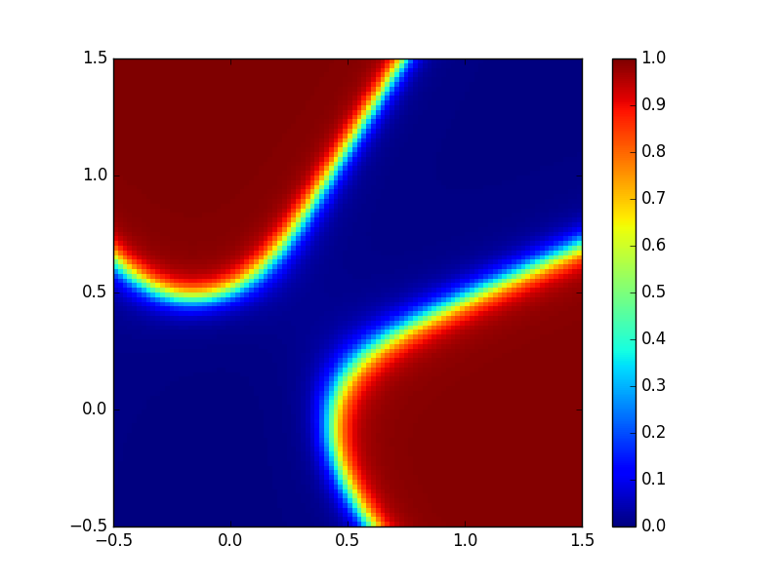
\includegraphics[scale=0.6]{images/xor_tanh_2_4.png}
\caption{2 couches cachées de 4 neurones-tanh}
\label{xor_tanh_2_4}
\end{center}
\end{figure}

L'apprentissage est donc concluant pour le XOR. Les résultats obtenus étant prometteurs, nous avons alors décidé de faire fonctionner l'algorithme sur les données MNIST.

MNIST est une base de données de chiffres écrits à la main assemblée par Yann Lecun. Cette base de donnée est constituée d'un ensemble de données d'apprentissage de 60.000 exemples et un ensemble de test constitué de 10.000 exemple. L'intersection de ces deux ensembles est nulle. Chaque exemple est donc une image d'une taille fixe d'un chiffre écrit à la main, centré. Le but est donc que notre algorithme puisse reconnaître les chiffres écrits.

Nous avons réalisé un premier apprentissage des données MNIST sur un réseau sans couche cachée totalement connecté (fully connected). Ce réseau dispose d'une entrée par pixel des images et de dix sorties, une par chiffre. Chaque entrée associe au pixel une valeur entre 0 et 255 correspondant à la nuance de gris du pixel (du blanc au noir). Un premier apprentissage est réalisé sur le réseau avec un calcul du gradient moyenné sur des batchs de 128 exemples. On calcule alors la précision du réseau de neurones sur l'ensemble complet d'apprentissage ainsi que sur l'ensemble de test tous les 2.000 exemples. La courbe d'évolution du coût lors de l'apprentissage est présentée figure \ref{mnist_apprentissage_128}. 

\begin{figure}[!h]
\begin{center}
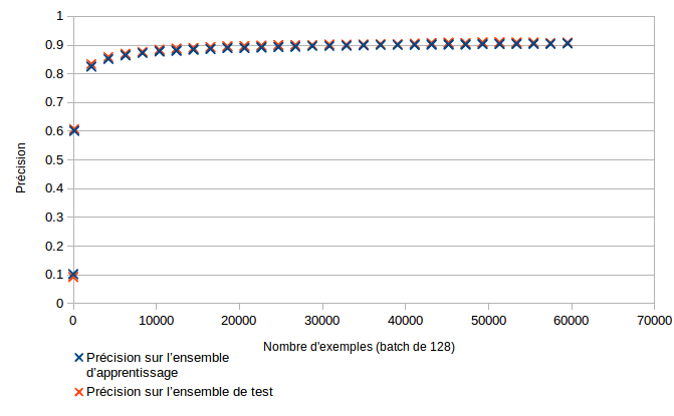
\includegraphics[scale=0.5]{images/mnist_apprentissage_128.png}
\caption{Précision en fonction du nombre d'exemples appris}
\label{mnist_apprentissage_128}
\end{center}
\end{figure}

On peut remarquer sur ces premiers résultats que la précision progresse très vite avant de plafonner autour des 90\% dès les 10.000 exemples utilisés. Nous avons obtenu une précision maximale de 90.83\% sur cette architecture neuronale très simpliste. Une précision plus importante pourrait être obtenue en ajoutant au moins une couche cachée au réseau. Cependant, le temps d'exécution avec cette première architecture (21.565 secondes soit plus de 6 heures), nous a montré qu'il serait impossible de réaliser un apprentissage en un temps raisonnable avec des architectures plus complexes.
\label{resultat_premiere_implementation}

\begin{figure}[!h]
\begin{center}
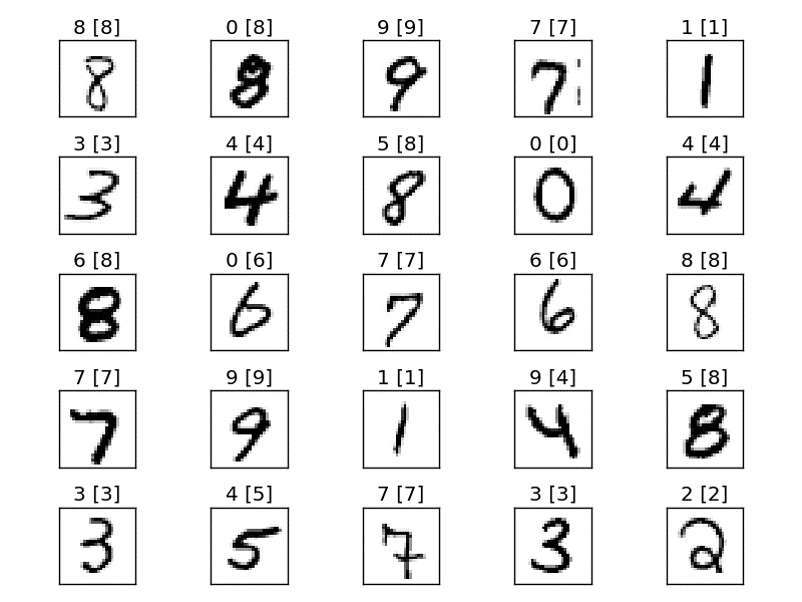
\includegraphics[scale=0.5]{images/mnist.png}
\caption{exemple de reconnaissance de caractères avec le réseau entrainé. caractère lu [caractère présenté]}
\label{mnist}
\end{center}
\end{figure}

\section{Conclusion}
Cette première implémentation intuitive permet ainsi d'obtenir des résultats très satisfaisants, allant jusqu'à 90\% de réussite sur le problème de	 MNIST. De plus, elle met en évidence le fonctionnement d'un réseau de neurones. Cependant, on remarque que les calculs ne sont pas du tout optimisés. Cela explique que le temps d'exécution devient rapidement très long. Dans l'exemple de l'application à l'ensemble de données MNIST, entraîner plusieurs fois le réseau sur l'ensemble d'apprentissage permettrait d'obtenir de bien meilleurs résultats, mais cela prendrait alors beaucoup trop de temps pour être véritablement envisageable.
Afin d'améliorer le temps de calcul et d'optimiser l'algorithme, nous nous sommes intéressés à une nouvelle approche des réseaux de neurones basée sur les graphes de calculs.
